\documentclass[1p]{elsarticle_modified}
%\bibliographystyle{elsarticle-num}

%\usepackage[colorlinks]{hyperref}
%\usepackage{abbrmath_seonhwa} %\Abb, \Ascr, \Acal ,\Abf, \Afrak
\usepackage{amsfonts}
\usepackage{amssymb}
\usepackage{amsmath}
\usepackage{amsthm}
\usepackage{scalefnt}
\usepackage{amsbsy}
\usepackage{kotex}
\usepackage{caption}
\usepackage{subfig}
\usepackage{color}
\usepackage{graphicx}
\usepackage{xcolor} %% white, black, red, green, blue, cyan, magenta, yellow
\usepackage{float}
\usepackage{setspace}
\usepackage{hyperref}

\usepackage{tikz}
\usetikzlibrary{arrows}

\usepackage{multirow}
\usepackage{array} % fixed length table
\usepackage{hhline}

%%%%%%%%%%%%%%%%%%%%%
\makeatletter
\renewcommand*\env@matrix[1][\arraystretch]{%
	\edef\arraystretch{#1}%
	\hskip -\arraycolsep
	\let\@ifnextchar\new@ifnextchar
	\array{*\c@MaxMatrixCols c}}
\makeatother %https://tex.stackexchange.com/questions/14071/how-can-i-increase-the-line-spacing-in-a-matrix
%%%%%%%%%%%%%%%

\usepackage[normalem]{ulem}

\newcommand{\msout}[1]{\ifmmode\text{\sout{\ensuremath{#1}}}\else\sout{#1}\fi}
%SOURCE: \msout is \stkout macro in https://tex.stackexchange.com/questions/20609/strikeout-in-math-mode

\newcommand{\cancel}[1]{
	\ifmmode
	{\color{red}\msout{#1}}
	\else
	{\color{red}\sout{#1}}
	\fi
}

\newcommand{\add}[1]{
	{\color{blue}\uwave{#1}}
}

\newcommand{\replace}[2]{
	\ifmmode
	{\color{red}\msout{#1}}{\color{blue}\uwave{#2}}
	\else
	{\color{red}\sout{#1}}{\color{blue}\uwave{#2}}
	\fi
}

\newcommand{\Sol}{\mathcal{S}} %segment
\newcommand{\D}{D} %diagram
\newcommand{\A}{\mathcal{A}} %arc


%%%%%%%%%%%%%%%%%%%%%%%%%%%%%5 test

\def\sl{\operatorname{\textup{SL}}(2,\Cbb)}
\def\psl{\operatorname{\textup{PSL}}(2,\Cbb)}
\def\quan{\mkern 1mu \triangleright \mkern 1mu}

\theoremstyle{definition}
\newtheorem{thm}{Theorem}[section]
\newtheorem{prop}[thm]{Proposition}
\newtheorem{lem}[thm]{Lemma}
\newtheorem{ques}[thm]{Question}
\newtheorem{cor}[thm]{Corollary}
\newtheorem{defn}[thm]{Definition}
\newtheorem{exam}[thm]{Example}
\newtheorem{rmk}[thm]{Remark}
\newtheorem{alg}[thm]{Algorithm}

\newcommand{\I}{\sqrt{-1}}
\begin{document}

%\begin{frontmatter}
%
%\title{Boundary parabolic representations of knots up to 8 crossings}
%
%%% Group authors per affiliation:
%\author{Yunhi Cho} 
%\address{Department of Mathematics, University of Seoul, Seoul, Korea}
%\ead{yhcho@uos.ac.kr}
%
%
%\author{Seonhwa Kim} %\fnref{s_kim}}
%\address{Center for Geometry and Physics, Institute for Basic Science, Pohang, 37673, Korea}
%\ead{ryeona17@ibs.re.kr}
%
%\author{Hyuk Kim}
%\address{Department of Mathematical Sciences, Seoul National University, Seoul 08826, Korea}
%\ead{hyukkim@snu.ac.kr}
%
%\author{Seokbeom Yoon}
%\address{Department of Mathematical Sciences, Seoul National University, Seoul, 08826,  Korea}
%\ead{sbyoon15@snu.ac.kr}
%
%\begin{abstract}
%We find all boundary parabolic representation of knots up to 8 crossings.
%
%\end{abstract}
%\begin{keyword}
%    \MSC[2010] 57M25 
%\end{keyword}
%
%\end{frontmatter}

%\linenumbers
%\tableofcontents
%
\newcommand\colored[1]{\textcolor{white}{\rule[-0.35ex]{0.8em}{1.4ex}}\kern-0.8em\color{red} #1}%
%\newcommand\colored[1]{\textcolor{white}{ #1}\kern-2.17ex	\textcolor{white}{ #1}\kern-1.81ex	\textcolor{white}{ #1}\kern-2.15ex\color{red}#1	}

{\Large $\underline{12n_{0453}~(K12n_{0453})}$}

\setlength{\tabcolsep}{10pt}
\renewcommand{\arraystretch}{1.6}
\vspace{1cm}\begin{tabular}{m{100pt}>{\centering\arraybackslash}m{274pt}}
\multirow{5}{120pt}{
	\centering
	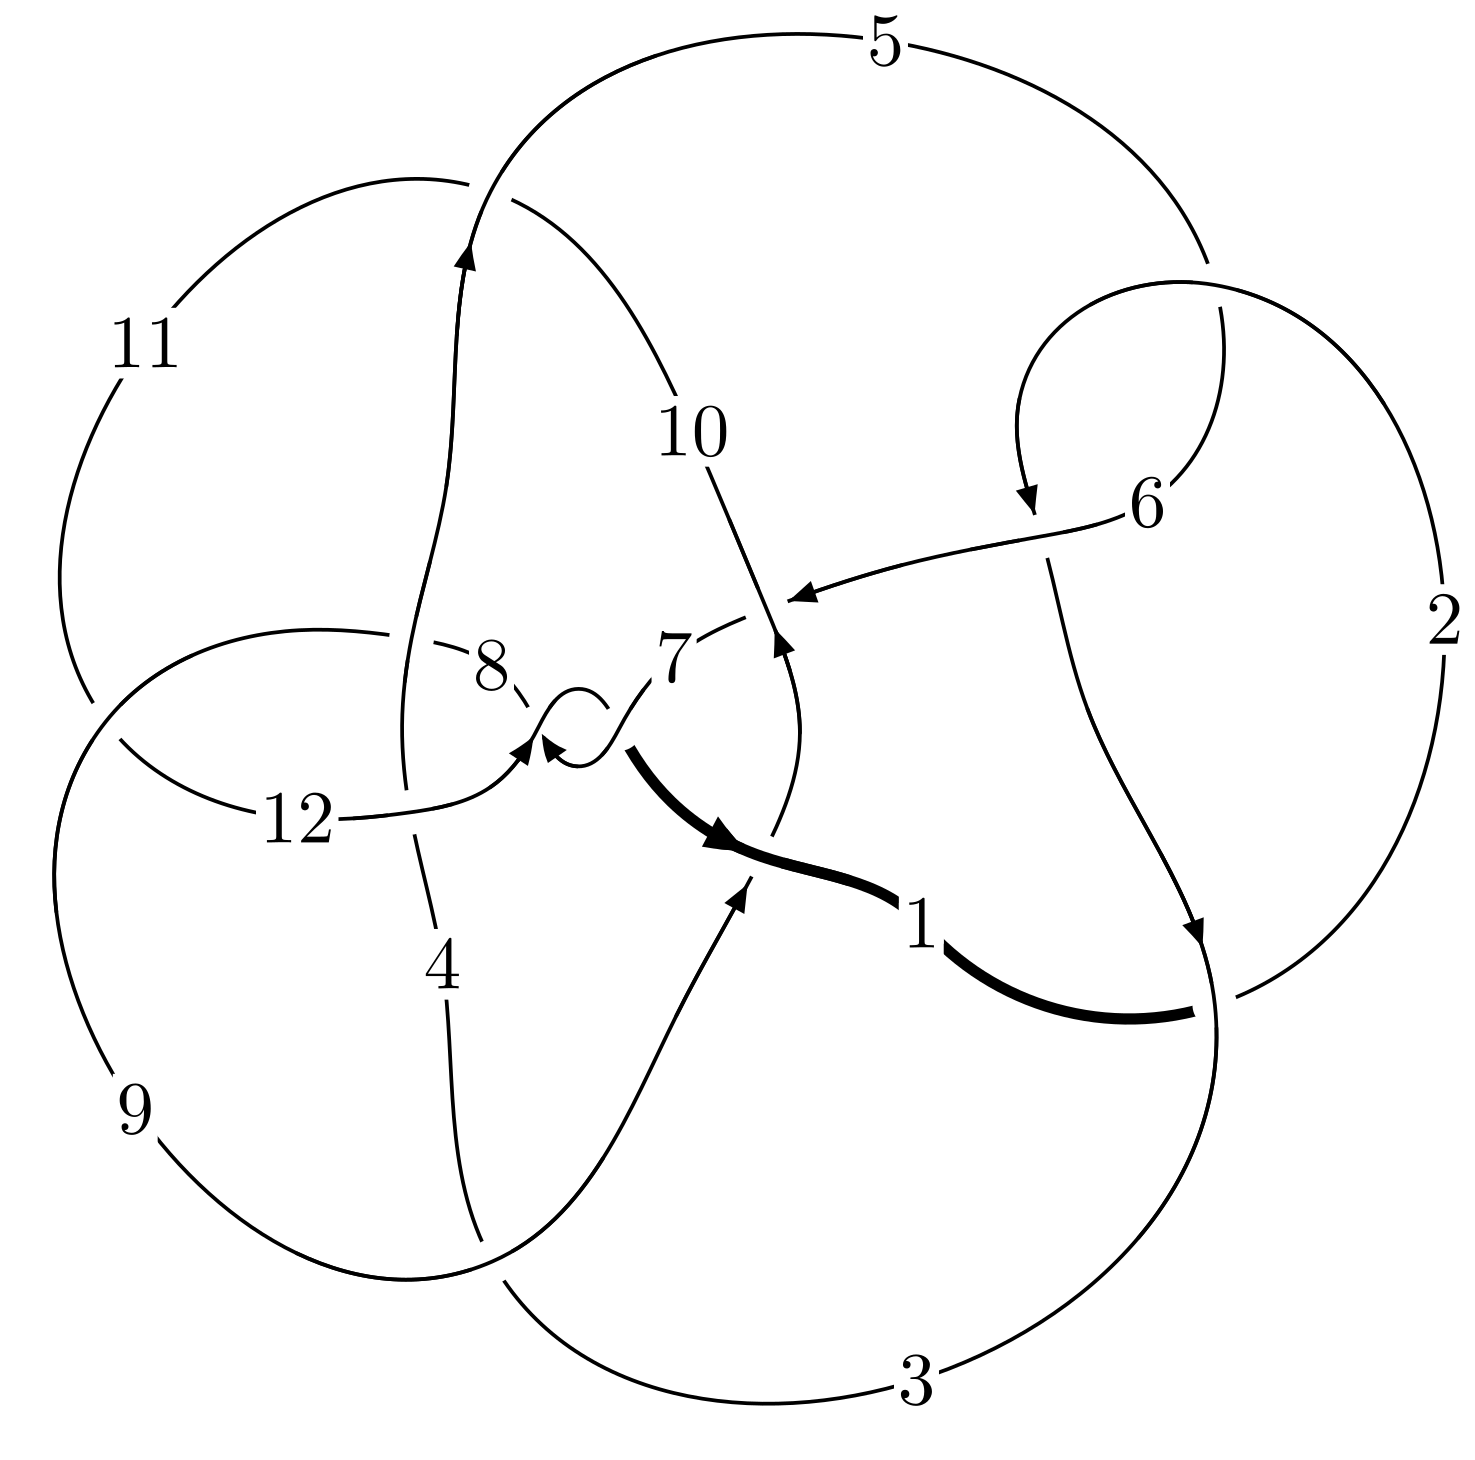
\includegraphics[width=112pt]{../../../GIT/diagram.site/Diagrams/png/2542_12n_0453.png}\\
\ \ \ A knot diagram\footnotemark}&
\allowdisplaybreaks
\textbf{Linearized knot diagam} \\
\cline{2-2}
 &
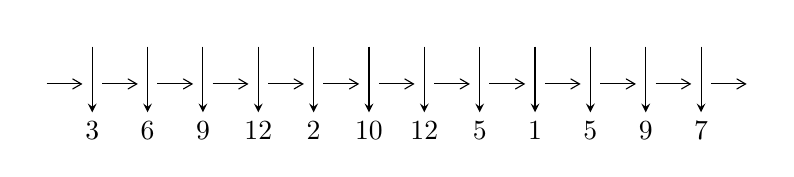
\begin{tikzpicture}[x=20pt, y=17pt]
	% nodes
	\node (C0) at (0, 0) {};
	\node (C1) at (1, 0) {};
	\node (C1U) at (1, +1) {};
	\node (C1D) at (1, -1) {3};

	\node (C2) at (2, 0) {};
	\node (C2U) at (2, +1) {};
	\node (C2D) at (2, -1) {6};

	\node (C3) at (3, 0) {};
	\node (C3U) at (3, +1) {};
	\node (C3D) at (3, -1) {9};

	\node (C4) at (4, 0) {};
	\node (C4U) at (4, +1) {};
	\node (C4D) at (4, -1) {12};

	\node (C5) at (5, 0) {};
	\node (C5U) at (5, +1) {};
	\node (C5D) at (5, -1) {2};

	\node (C6) at (6, 0) {};
	\node (C6U) at (6, +1) {};
	\node (C6D) at (6, -1) {10};

	\node (C7) at (7, 0) {};
	\node (C7U) at (7, +1) {};
	\node (C7D) at (7, -1) {12};

	\node (C8) at (8, 0) {};
	\node (C8U) at (8, +1) {};
	\node (C8D) at (8, -1) {5};

	\node (C9) at (9, 0) {};
	\node (C9U) at (9, +1) {};
	\node (C9D) at (9, -1) {1};

	\node (C10) at (10, 0) {};
	\node (C10U) at (10, +1) {};
	\node (C10D) at (10, -1) {5};

	\node (C11) at (11, 0) {};
	\node (C11U) at (11, +1) {};
	\node (C11D) at (11, -1) {9};

	\node (C12) at (12, 0) {};
	\node (C12U) at (12, +1) {};
	\node (C12D) at (12, -1) {7};
	\node (C13) at (13, 0) {};

	% arrows
	\draw[->,>={angle 60}]
	(C0) edge (C1) (C1) edge (C2) (C2) edge (C3) (C3) edge (C4) (C4) edge (C5) (C5) edge (C6) (C6) edge (C7) (C7) edge (C8) (C8) edge (C9) (C9) edge (C10) (C10) edge (C11) (C11) edge (C12) (C12) edge (C13) ;	\draw[->,>=stealth]
	(C1U) edge (C1D) (C2U) edge (C2D) (C3U) edge (C3D) (C4U) edge (C4D) (C5U) edge (C5D) (C6U) edge (C6D) (C7U) edge (C7D) (C8U) edge (C8D) (C9U) edge (C9D) (C10U) edge (C10D) (C11U) edge (C11D) (C12U) edge (C12D) ;
	\end{tikzpicture} \\
\hhline{~~} \\& 
\textbf{Solving Sequence} \\ \cline{2-2} 
 &
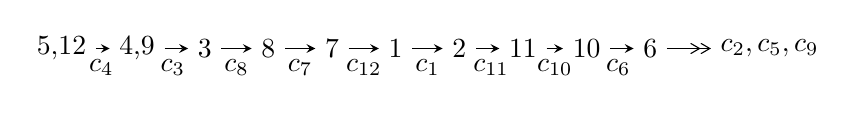
\begin{tikzpicture}[x=23pt, y=7pt]
	% node
	\node (A0) at (-1/8, 0) {5,12};
	\node (A1) at (17/16, 0) {4,9};
	\node (A2) at (17/8, 0) {3};
	\node (A3) at (25/8, 0) {8};
	\node (A4) at (33/8, 0) {7};
	\node (A5) at (41/8, 0) {1};
	\node (A6) at (49/8, 0) {2};
	\node (A7) at (57/8, 0) {11};
	\node (A8) at (65/8, 0) {10};
	\node (A9) at (73/8, 0) {6};
	\node (C1) at (1/2, -1) {$c_{4}$};
	\node (C2) at (13/8, -1) {$c_{3}$};
	\node (C3) at (21/8, -1) {$c_{8}$};
	\node (C4) at (29/8, -1) {$c_{7}$};
	\node (C5) at (37/8, -1) {$c_{12}$};
	\node (C6) at (45/8, -1) {$c_{1}$};
	\node (C7) at (53/8, -1) {$c_{11}$};
	\node (C8) at (61/8, -1) {$c_{10}$};
	\node (C9) at (69/8, -1) {$c_{6}$};
	\node (A10) at (11, 0) {$c_{2},c_{5},c_{9}$};

	% edge
	\draw[->,>=stealth]	
	(A0) edge (A1) (A1) edge (A2) (A2) edge (A3) (A3) edge (A4) (A4) edge (A5) (A5) edge (A6) (A6) edge (A7) (A7) edge (A8) (A8) edge (A9) ;
	\draw[->>,>={angle 60}]	
	(A9) edge (A10);
\end{tikzpicture} \\ 

\end{tabular} \\

\footnotetext{
The image of knot diagram is generated by the software ``\textbf{Draw programme}" developed by Andrew Bartholomew(\url{http://www.layer8.co.uk/maths/draw/index.htm\#Running-draw}), where we modified some parts for our purpose(\url{https://github.com/CATsTAILs/LinksPainter}).
}\phantom \\ \newline 
\centering \textbf{Ideals for irreducible components\footnotemark of $X_{\text{par}}$} 
 
\begin{align*}
I^u_{1}&=\langle 
b- u,\;-5.24830\times10^{36} u^{34}+3.76703\times10^{36} u^{33}+\cdots+1.56072\times10^{36} a-5.62245\times10^{36},\\
\phantom{I^u_{1}}&\phantom{= \langle  }u^{35}- u^{34}+\cdots+3 u-1\rangle \\
I^u_{2}&=\langle 
2.26126\times10^{120} u^{43}-6.93064\times10^{119} u^{42}+\cdots+1.57860\times10^{123} b-2.38102\times10^{124},\\
\phantom{I^u_{2}}&\phantom{= \langle  }-6.59277\times10^{123} u^{43}+5.75046\times10^{123} u^{42}+\cdots+1.55634\times10^{127} a+1.14048\times10^{128},\\
\phantom{I^u_{2}}&\phantom{= \langle  }u^{44}- u^{43}+\cdots-34132 u+9859\rangle \\
I^u_{3}&=\langle 
b+u,\;-541775388218 u^{21}+737506675481 u^{20}+\cdots+532384024235 a-996909356925,\\
\phantom{I^u_{3}}&\phantom{= \langle  }u^{22}- u^{21}+\cdots-13 u^3-1\rangle \\
\\
\end{align*}
\raggedright * 3 irreducible components of $\dim_{\mathbb{C}}=0$, with total 101 representations.\\
\footnotetext{All coefficients of polynomials are rational numbers. But the coefficients are sometimes approximated in decimal forms when there is not enough margin.}
\newpage
\renewcommand{\arraystretch}{1}
\centering \section*{I. $I^u_{1}= \langle b- u,\;-5.25\times10^{36} u^{34}+3.77\times10^{36} u^{33}+\cdots+1.56\times10^{36} a-5.62\times10^{36},\;u^{35}- u^{34}+\cdots+3 u-1 \rangle$}
\flushleft \textbf{(i) Arc colorings}\\
\begin{tabular}{m{7pt} m{180pt} m{7pt} m{180pt} }
\flushright $a_{5}=$&$\begin{pmatrix}1\\0\end{pmatrix}$ \\
\flushright $a_{12}=$&$\begin{pmatrix}0\\u\end{pmatrix}$ \\
\flushright $a_{4}=$&$\begin{pmatrix}1\\- u^2\end{pmatrix}$ \\
\flushright $a_{9}=$&$\begin{pmatrix}3.36274 u^{34}-2.41365 u^{33}+\cdots-1.77064 u+3.60247\\u\end{pmatrix}$ \\
\flushright $a_{3}=$&$\begin{pmatrix}-1.50962 u^{34}+0.0976335 u^{33}+\cdots+5.85679 u-2.87425\\-0.390812 u^{34}+0.123541 u^{33}+\cdots+1.97017 u-0.973088\end{pmatrix}$ \\
\flushright $a_{8}=$&$\begin{pmatrix}3.36274 u^{34}-2.41365 u^{33}+\cdots-0.770637 u+3.60247\\u\end{pmatrix}$ \\
\flushright $a_{7}=$&$\begin{pmatrix}3.36274 u^{34}-2.41365 u^{33}+\cdots-0.770637 u+3.60247\\-0.973088 u^{34}+0.582276 u^{33}+\cdots+0.484542 u-0.949096\end{pmatrix}$ \\
\flushright $a_{1}=$&$\begin{pmatrix}-2.45768 u^{34}+1.11553 u^{33}+\cdots+6.33799 u-4.06168\\0.000350385 u^{34}-0.0450612 u^{33}+\cdots-1.08421 u+0.393051\end{pmatrix}$ \\
\flushright $a_{2}=$&$\begin{pmatrix}0.302246 u^{34}+0.208870 u^{33}+\cdots-6.15873 u+2.00069\\-1.63367 u^{34}+0.497640 u^{33}+\cdots+4.44370 u-2.88225\end{pmatrix}$ \\
\flushright $a_{11}=$&$\begin{pmatrix}0.511505 u^{34}+0.0490164 u^{33}+\cdots-7.36890 u+2.16349\\0.973088 u^{34}-0.582276 u^{33}+\cdots+1.51546 u+0.949096\end{pmatrix}$ \\
\flushright $a_{10}=$&$\begin{pmatrix}1.48459 u^{34}-0.533259 u^{33}+\cdots-5.85345 u+3.11258\\0.973088 u^{34}-0.582276 u^{33}+\cdots+1.51546 u+0.949096\end{pmatrix}$ \\
\flushright $a_{6}=$&$\begin{pmatrix}0.778426 u^{34}+0.0389110 u^{33}+\cdots-3.48404 u+2.16125\\-2.31610 u^{34}+0.760393 u^{33}+\cdots+7.17608 u-4.33272\end{pmatrix}$\\&\end{tabular}
\flushleft \textbf{(ii) Obstruction class $= -1$}\\~\\
\flushleft \textbf{(iii) Cusp Shapes $= 0.563437 u^{34}+0.739161 u^{33}+\cdots-7.54274 u-12.9075$}\\~\\
\newpage\renewcommand{\arraystretch}{1}
\flushleft \textbf{(iv) u-Polynomials at the component}\newline \\
\begin{tabular}{m{50pt}|m{274pt}}
Crossings & \hspace{64pt}u-Polynomials at each crossing \\
\hline $$\begin{aligned}c_{1}\end{aligned}$$&$\begin{aligned}
&u^{35}+18 u^{34}+\cdots+268 u+16
\end{aligned}$\\
\hline $$\begin{aligned}c_{2},c_{5}\end{aligned}$$&$\begin{aligned}
&u^{35}+8 u^{34}+\cdots+42 u+4
\end{aligned}$\\
\hline $$\begin{aligned}c_{3},c_{10}\end{aligned}$$&$\begin{aligned}
&u^{35}-3 u^{33}+\cdots-2 u+5
\end{aligned}$\\
\hline $$\begin{aligned}c_{4},c_{8}\end{aligned}$$&$\begin{aligned}
&u^{35}+u^{34}+\cdots+3 u+1
\end{aligned}$\\
\hline $$\begin{aligned}c_{6},c_{9}\end{aligned}$$&$\begin{aligned}
&u^{35}- u^{34}+\cdots-2 u+1
\end{aligned}$\\
\hline $$\begin{aligned}c_{7},c_{12}\end{aligned}$$&$\begin{aligned}
&u^{35}+24 u^{34}+\cdots+39936 u+2048
\end{aligned}$\\
\hline $$\begin{aligned}c_{11}\end{aligned}$$&$\begin{aligned}
&u^{35}-23 u^{34}+\cdots-230 u+1300
\end{aligned}$\\
\hline
\end{tabular}\\~\\
\newpage\renewcommand{\arraystretch}{1}
\flushleft \textbf{(v) Riley Polynomials at the component}\newline \\
\begin{tabular}{m{50pt}|m{274pt}}
Crossings & \hspace{64pt}Riley Polynomials at each crossing \\
\hline $$\begin{aligned}c_{1}\end{aligned}$$&$\begin{aligned}
&y^{35}+2 y^{34}+\cdots+40048 y-256
\end{aligned}$\\
\hline $$\begin{aligned}c_{2},c_{5}\end{aligned}$$&$\begin{aligned}
&y^{35}-18 y^{34}+\cdots+268 y-16
\end{aligned}$\\
\hline $$\begin{aligned}c_{3},c_{10}\end{aligned}$$&$\begin{aligned}
&y^{35}-6 y^{34}+\cdots+434 y-25
\end{aligned}$\\
\hline $$\begin{aligned}c_{4},c_{8}\end{aligned}$$&$\begin{aligned}
&y^{35}-47 y^{34}+\cdots+13 y-1
\end{aligned}$\\
\hline $$\begin{aligned}c_{6},c_{9}\end{aligned}$$&$\begin{aligned}
&y^{35}+3 y^{34}+\cdots-2 y-1
\end{aligned}$\\
\hline $$\begin{aligned}c_{7},c_{12}\end{aligned}$$&$\begin{aligned}
&y^{35}+16 y^{34}+\cdots+47185920 y-4194304
\end{aligned}$\\
\hline $$\begin{aligned}c_{11}\end{aligned}$$&$\begin{aligned}
&y^{35}-23 y^{34}+\cdots+9249100 y-1690000
\end{aligned}$\\
\hline
\end{tabular}\\~\\
\newpage\flushleft \textbf{(vi) Complex Volumes and Cusp Shapes}
$$\begin{array}{c|c|c}  
\text{Solutions to }I^u_{1}& \I (\text{vol} + \sqrt{-1}CS) & \text{Cusp shape}\\
 \hline 
\begin{aligned}
u &= \phantom{-}0.955967 + 0.450664 I \\
a &= -0.277341 + 1.028180 I \\
b &= \phantom{-}0.955967 + 0.450664 I\end{aligned}
 & \phantom{-}0.32153 + 2.91618 I & -4.71539 - 0.02368 I \\ \hline\begin{aligned}
u &= \phantom{-}0.955967 - 0.450664 I \\
a &= -0.277341 - 1.028180 I \\
b &= \phantom{-}0.955967 - 0.450664 I\end{aligned}
 & \phantom{-}0.32153 - 2.91618 I & -4.71539 + 0.02368 I \\ \hline\begin{aligned}
u &= -0.603532 + 0.339224 I \\
a &= -0.087049 - 1.096610 I \\
b &= -0.603532 + 0.339224 I\end{aligned}
 & -1.37493 - 3.82893 I & -14.7554 + 5.1588 I \\ \hline\begin{aligned}
u &= -0.603532 - 0.339224 I \\
a &= -0.087049 + 1.096610 I \\
b &= -0.603532 - 0.339224 I\end{aligned}
 & -1.37493 + 3.82893 I & -14.7554 - 5.1588 I \\ \hline\begin{aligned}
u &= \phantom{-}0.505207 + 0.466803 I \\
a &= -1.53217 - 2.19035 I \\
b &= \phantom{-}0.505207 + 0.466803 I\end{aligned}
 & \phantom{-}3.54205 + 7.35026 I & -11.99203 - 4.50938 I \\ \hline\begin{aligned}
u &= \phantom{-}0.505207 - 0.466803 I \\
a &= -1.53217 + 2.19035 I \\
b &= \phantom{-}0.505207 - 0.466803 I\end{aligned}
 & \phantom{-}3.54205 - 7.35026 I & -11.99203 + 4.50938 I \\ \hline\begin{aligned}
u &= -0.639207 + 0.204758 I \\
a &= -0.14927 + 1.74146 I \\
b &= -0.639207 + 0.204758 I\end{aligned}
 & \phantom{-}3.60027 + 1.54452 I & -7.64624 - 4.60913 I \\ \hline\begin{aligned}
u &= -0.639207 - 0.204758 I \\
a &= -0.14927 - 1.74146 I \\
b &= -0.639207 - 0.204758 I\end{aligned}
 & \phantom{-}3.60027 - 1.54452 I & -7.64624 + 4.60913 I \\ \hline\begin{aligned}
u &= \phantom{-}0.373896 + 0.520116 I \\
a &= \phantom{-}1.270260 + 0.311437 I \\
b &= \phantom{-}0.373896 + 0.520116 I\end{aligned}
 & \phantom{-}0.95580 - 4.75953 I & -9.19791 + 7.90177 I \\ \hline\begin{aligned}
u &= \phantom{-}0.373896 - 0.520116 I \\
a &= \phantom{-}1.270260 - 0.311437 I \\
b &= \phantom{-}0.373896 - 0.520116 I\end{aligned}
 & \phantom{-}0.95580 + 4.75953 I & -9.19791 - 7.90177 I\\
 \hline 
 \end{array}$$\newpage$$\begin{array}{c|c|c}  
\text{Solutions to }I^u_{1}& \I (\text{vol} + \sqrt{-1}CS) & \text{Cusp shape}\\
 \hline 
\begin{aligned}
u &= -0.558191 + 0.285053 I \\
a &= \phantom{-}1.18752 - 2.42194 I \\
b &= -0.558191 + 0.285053 I\end{aligned}
 & \phantom{-}4.88354 - 2.69019 I & -10.47730 + 0.12447 I \\ \hline\begin{aligned}
u &= -0.558191 - 0.285053 I \\
a &= \phantom{-}1.18752 + 2.42194 I \\
b &= -0.558191 - 0.285053 I\end{aligned}
 & \phantom{-}4.88354 + 2.69019 I & -10.47730 - 0.12447 I \\ \hline\begin{aligned}
u &= \phantom{-}0.605489 + 0.009295 I \\
a &= \phantom{-}0.206739 + 0.573796 I \\
b &= \phantom{-}0.605489 + 0.009295 I\end{aligned}
 & -0.426536 + 0.312778 I & -12.16336 + 0.78895 I \\ \hline\begin{aligned}
u &= \phantom{-}0.605489 - 0.009295 I \\
a &= \phantom{-}0.206739 - 0.573796 I \\
b &= \phantom{-}0.605489 - 0.009295 I\end{aligned}
 & -0.426536 - 0.312778 I & -12.16336 - 0.78895 I \\ \hline\begin{aligned}
u &= -0.177738 + 0.486118 I \\
a &= -0.17737 - 1.74965 I \\
b &= -0.177738 + 0.486118 I\end{aligned}
 & -2.39864 + 1.51734 I & -15.0669 - 4.1108 I \\ \hline\begin{aligned}
u &= -0.177738 - 0.486118 I \\
a &= -0.17737 + 1.74965 I \\
b &= -0.177738 - 0.486118 I\end{aligned}
 & -2.39864 - 1.51734 I & -15.0669 + 4.1108 I \\ \hline\begin{aligned}
u &= \phantom{-}0.057585 + 0.464773 I \\
a &= -2.70671 - 1.34166 I \\
b &= \phantom{-}0.057585 + 0.464773 I\end{aligned}
 & \phantom{-}1.72575 + 1.86389 I & -7.37932 + 5.72849 I \\ \hline\begin{aligned}
u &= \phantom{-}0.057585 - 0.464773 I \\
a &= -2.70671 + 1.34166 I \\
b &= \phantom{-}0.057585 - 0.464773 I\end{aligned}
 & \phantom{-}1.72575 - 1.86389 I & -7.37932 - 5.72849 I \\ \hline\begin{aligned}
u &= \phantom{-}1.54010 + 0.38619 I \\
a &= -0.729617 + 0.149966 I \\
b &= \phantom{-}1.54010 + 0.38619 I\end{aligned}
 & -1.11453 - 0.96016 I & \phantom{-0.000000 } 0 \\ \hline\begin{aligned}
u &= \phantom{-}1.54010 - 0.38619 I \\
a &= -0.729617 - 0.149966 I \\
b &= \phantom{-}1.54010 - 0.38619 I\end{aligned}
 & -1.11453 + 0.96016 I & \phantom{-0.000000 } 0\\
 \hline 
 \end{array}$$\newpage$$\begin{array}{c|c|c}  
\text{Solutions to }I^u_{1}& \I (\text{vol} + \sqrt{-1}CS) & \text{Cusp shape}\\
 \hline 
\begin{aligned}
u &= -1.58422 + 0.48939 I \\
a &= \phantom{-}0.844245 + 0.075878 I \\
b &= -1.58422 + 0.48939 I\end{aligned}
 & -0.30923 + 6.97118 I & \phantom{-0.000000 } 0 \\ \hline\begin{aligned}
u &= -1.58422 - 0.48939 I \\
a &= \phantom{-}0.844245 - 0.075878 I \\
b &= -1.58422 - 0.48939 I\end{aligned}
 & -0.30923 - 6.97118 I & \phantom{-0.000000 } 0 \\ \hline\begin{aligned}
u &= \phantom{-}0.339571\phantom{ +0.000000I} \\
a &= \phantom{-}0.730904\phantom{ +0.000000I} \\
b &= \phantom{-}0.339571\phantom{ +0.000000I}\end{aligned}
 & -0.605268\phantom{ +0.000000I} & -16.1480\phantom{ +0.000000I} \\ \hline\begin{aligned}
u &= \phantom{-}1.72430 + 0.03737 I \\
a &= -0.913428 - 0.274991 I \\
b &= \phantom{-}1.72430 + 0.03737 I\end{aligned}
 & -5.06642 - 3.71082 I & \phantom{-0.000000 } 0 \\ \hline\begin{aligned}
u &= \phantom{-}1.72430 - 0.03737 I \\
a &= -0.913428 + 0.274991 I \\
b &= \phantom{-}1.72430 - 0.03737 I\end{aligned}
 & -5.06642 + 3.71082 I & \phantom{-0.000000 } 0 \\ \hline\begin{aligned}
u &= -1.75744 + 0.08760 I \\
a &= \phantom{-}0.995064 - 0.291635 I \\
b &= -1.75744 + 0.08760 I\end{aligned}
 & -7.51086 + 9.54692 I & \phantom{-0.000000 } 0 \\ \hline\begin{aligned}
u &= -1.75744 - 0.08760 I \\
a &= \phantom{-}0.995064 + 0.291635 I \\
b &= -1.75744 - 0.08760 I\end{aligned}
 & -7.51086 - 9.54692 I & \phantom{-0.000000 } 0 \\ \hline\begin{aligned}
u &= \phantom{-}1.70176 + 0.47815 I \\
a &= -1.051060 + 0.162856 I \\
b &= \phantom{-}1.70176 + 0.47815 I\end{aligned}
 & -7.79536 - 8.25620 I & \phantom{-0.000000 } 0 \\ \hline\begin{aligned}
u &= \phantom{-}1.70176 - 0.47815 I \\
a &= -1.051060 - 0.162856 I \\
b &= \phantom{-}1.70176 - 0.47815 I\end{aligned}
 & -7.79536 + 8.25620 I & \phantom{-0.000000 } 0 \\ \hline\begin{aligned}
u &= -1.71391 + 0.54641 I \\
a &= \phantom{-}1.082860 + 0.037259 I \\
b &= -1.71391 + 0.54641 I\end{aligned}
 & -1.90251 + 11.15310 I & \phantom{-0.000000 } 0\\
 \hline 
 \end{array}$$\newpage$$\begin{array}{c|c|c}  
\text{Solutions to }I^u_{1}& \I (\text{vol} + \sqrt{-1}CS) & \text{Cusp shape}\\
 \hline 
\begin{aligned}
u &= -1.71391 - 0.54641 I \\
a &= \phantom{-}1.082860 - 0.037259 I \\
b &= -1.71391 - 0.54641 I\end{aligned}
 & -1.90251 - 11.15310 I & \phantom{-0.000000 } 0 \\ \hline\begin{aligned}
u &= \phantom{-}1.74961 + 0.55030 I \\
a &= -1.143750 + 0.033525 I \\
b &= \phantom{-}1.74961 + 0.55030 I\end{aligned}
 & -4.1343 - 16.7869 I & \phantom{-0.000000 } 0 \\ \hline\begin{aligned}
u &= \phantom{-}1.74961 - 0.55030 I \\
a &= -1.143750 - 0.033525 I \\
b &= \phantom{-}1.74961 - 0.55030 I\end{aligned}
 & -4.1343 + 16.7869 I & \phantom{-0.000000 } 0 \\ \hline\begin{aligned}
u &= -1.84947 + 0.03525 I \\
a &= \phantom{-}0.815630 + 0.068482 I \\
b &= -1.84947 + 0.03525 I\end{aligned}
 & -11.47940 - 0.02354 I & \phantom{-0.000000 } 0 \\ \hline\begin{aligned}
u &= -1.84947 - 0.03525 I \\
a &= \phantom{-}0.815630 - 0.068482 I \\
b &= -1.84947 - 0.03525 I\end{aligned}
 & -11.47940 + 0.02354 I & \phantom{-0.000000 } 0\\
 \hline 
 \end{array}$$\newpage\newpage\renewcommand{\arraystretch}{1}
\centering \section*{II. $I^u_{2}= \langle 2.26\times10^{120} u^{43}-6.93\times10^{119} u^{42}+\cdots+1.58\times10^{123} b-2.38\times10^{124},\;-6.59\times10^{123} u^{43}+5.75\times10^{123} u^{42}+\cdots+1.56\times10^{127} a+1.14\times10^{128},\;u^{44}- u^{43}+\cdots-34132 u+9859 \rangle$}
\flushleft \textbf{(i) Arc colorings}\\
\begin{tabular}{m{7pt} m{180pt} m{7pt} m{180pt} }
\flushright $a_{5}=$&$\begin{pmatrix}1\\0\end{pmatrix}$ \\
\flushright $a_{12}=$&$\begin{pmatrix}0\\u\end{pmatrix}$ \\
\flushright $a_{4}=$&$\begin{pmatrix}1\\- u^2\end{pmatrix}$ \\
\flushright $a_{9}=$&$\begin{pmatrix}0.000423608 u^{43}-0.000369486 u^{42}+\cdots+1.13379 u-7.32800\\-0.00143245 u^{43}+0.000439038 u^{42}+\cdots-35.5630 u+15.0831\end{pmatrix}$ \\
\flushright $a_{3}=$&$\begin{pmatrix}-0.000366681 u^{43}+6.86484\times10^{-6} u^{42}+\cdots+0.722864 u+4.29414\\-0.000979566 u^{43}+0.000158000 u^{42}+\cdots-38.9308 u+18.6302\end{pmatrix}$ \\
\flushright $a_{8}=$&$\begin{pmatrix}-0.00100884 u^{43}+0.0000695518 u^{42}+\cdots-34.4292 u+7.75514\\-0.00143245 u^{43}+0.000439038 u^{42}+\cdots-35.5630 u+15.0831\end{pmatrix}$ \\
\flushright $a_{7}=$&$\begin{pmatrix}-0.00100884 u^{43}+0.0000695518 u^{42}+\cdots-34.4292 u+7.75514\\-0.000519378 u^{43}+0.000227604 u^{42}+\cdots-13.4493 u+5.82268\end{pmatrix}$ \\
\flushright $a_{1}=$&$\begin{pmatrix}-0.00111027 u^{43}+0.000170982 u^{42}+\cdots-24.7199 u+11.2172\\0.0000227599 u^{43}+0.0000793547 u^{42}+\cdots+7.51625 u+0.662428\end{pmatrix}$ \\
\flushright $a_{2}=$&$\begin{pmatrix}-0.00106771 u^{43}+0.000531820 u^{42}+\cdots-15.1776 u+15.0692\\-0.00135172 u^{43}+0.000249506 u^{42}+\cdots-22.2369 u+10.6788\end{pmatrix}$ \\
\flushright $a_{11}=$&$\begin{pmatrix}-0.00104245 u^{43}+0.000171126 u^{42}+\cdots-18.5615 u+10.9112\\0.00126241 u^{43}-0.0000513188 u^{42}+\cdots+29.6839 u-12.2055\end{pmatrix}$ \\
\flushright $a_{10}=$&$\begin{pmatrix}0.000219960 u^{43}+0.000119807 u^{42}+\cdots+11.1224 u-1.29427\\0.00126241 u^{43}-0.0000513188 u^{42}+\cdots+29.6839 u-12.2055\end{pmatrix}$ \\
\flushright $a_{6}=$&$\begin{pmatrix}0.000928242 u^{43}-0.000395266 u^{42}+\cdots+6.92574 u-13.5888\\0.00136897 u^{43}-0.000507756 u^{42}+\cdots+27.5784 u-15.4736\end{pmatrix}$\\&\end{tabular}
\flushleft \textbf{(ii) Obstruction class $= -1$}\\~\\
\flushleft \textbf{(iii) Cusp Shapes $= 0.00924417 u^{43}-0.00117823 u^{42}+\cdots+253.150 u-126.267$}\\~\\
\newpage\renewcommand{\arraystretch}{1}
\flushleft \textbf{(iv) u-Polynomials at the component}\newline \\
\begin{tabular}{m{50pt}|m{274pt}}
Crossings & \hspace{64pt}u-Polynomials at each crossing \\
\hline $$\begin{aligned}c_{1}\end{aligned}$$&$\begin{aligned}
&(u^{11}+5 u^{10}+\cdots+2 u+1)^{4}
\end{aligned}$\\
\hline $$\begin{aligned}c_{2},c_{5}\end{aligned}$$&$\begin{aligned}
&(u^{11}- u^{10}-2 u^9+3 u^8+2 u^7-4 u^6+3 u^4- u^3- u^2+1)^4
\end{aligned}$\\
\hline $$\begin{aligned}c_{3},c_{10}\end{aligned}$$&$\begin{aligned}
&u^{44}- u^{43}+\cdots+910 u+19909
\end{aligned}$\\
\hline $$\begin{aligned}c_{4},c_{8}\end{aligned}$$&$\begin{aligned}
&u^{44}+u^{43}+\cdots+34132 u+9859
\end{aligned}$\\
\hline $$\begin{aligned}c_{6},c_{9}\end{aligned}$$&$\begin{aligned}
&u^{44}+9 u^{43}+\cdots+332 u+43
\end{aligned}$\\
\hline $$\begin{aligned}c_{7},c_{12}\end{aligned}$$&$\begin{aligned}
&(u^2- u+1)^{22}
\end{aligned}$\\
\hline $$\begin{aligned}c_{11}\end{aligned}$$&$\begin{aligned}
&(u^{11}+9 u^{10}+\cdots+10 u-1)^{4}
\end{aligned}$\\
\hline
\end{tabular}\\~\\
\newpage\renewcommand{\arraystretch}{1}
\flushleft \textbf{(v) Riley Polynomials at the component}\newline \\
\begin{tabular}{m{50pt}|m{274pt}}
Crossings & \hspace{64pt}Riley Polynomials at each crossing \\
\hline $$\begin{aligned}c_{1}\end{aligned}$$&$\begin{aligned}
&(y^{11}+3 y^{10}+\cdots-10 y-1)^{4}
\end{aligned}$\\
\hline $$\begin{aligned}c_{2},c_{5}\end{aligned}$$&$\begin{aligned}
&(y^{11}-5 y^{10}+\cdots+2 y-1)^{4}
\end{aligned}$\\
\hline $$\begin{aligned}c_{3},c_{10}\end{aligned}$$&$\begin{aligned}
&y^{44}-21 y^{43}+\cdots-17790568 y+396368281
\end{aligned}$\\
\hline $$\begin{aligned}c_{4},c_{8}\end{aligned}$$&$\begin{aligned}
&y^{44}-45 y^{43}+\cdots-3052479256 y+97199881
\end{aligned}$\\
\hline $$\begin{aligned}c_{6},c_{9}\end{aligned}$$&$\begin{aligned}
&y^{44}+11 y^{43}+\cdots+25828 y+1849
\end{aligned}$\\
\hline $$\begin{aligned}c_{7},c_{12}\end{aligned}$$&$\begin{aligned}
&(y^2+y+1)^{22}
\end{aligned}$\\
\hline $$\begin{aligned}c_{11}\end{aligned}$$&$\begin{aligned}
&(y^{11}-21 y^{10}+\cdots+66 y-1)^{4}
\end{aligned}$\\
\hline
\end{tabular}\\~\\
\newpage\flushleft \textbf{(vi) Complex Volumes and Cusp Shapes}
$$\begin{array}{c|c|c}  
\text{Solutions to }I^u_{2}& \I (\text{vol} + \sqrt{-1}CS) & \text{Cusp shape}\\
 \hline 
\begin{aligned}
u &= -0.146600 + 1.027860 I \\
a &= \phantom{-}0.0175660 + 0.1231610 I \\
b &= \phantom{-}0.876184 + 0.235814 I\end{aligned}
 & -1.55223 + 2.02988 I & -15.8143 - 3.4641 I \\ \hline\begin{aligned}
u &= -0.146600 - 1.027860 I \\
a &= \phantom{-}0.0175660 - 0.1231610 I \\
b &= \phantom{-}0.876184 - 0.235814 I\end{aligned}
 & -1.55223 - 2.02988 I & -15.8143 + 3.4641 I \\ \hline\begin{aligned}
u &= \phantom{-}0.876184 + 0.235814 I \\
a &= -0.137463 + 0.036996 I \\
b &= -0.146600 + 1.027860 I\end{aligned}
 & -1.55223 + 2.02988 I & -15.8143 - 3.4641 I \\ \hline\begin{aligned}
u &= \phantom{-}0.876184 - 0.235814 I \\
a &= -0.137463 - 0.036996 I \\
b &= -0.146600 - 1.027860 I\end{aligned}
 & -1.55223 - 2.02988 I & -15.8143 + 3.4641 I \\ \hline\begin{aligned}
u &= \phantom{-}0.834580 + 0.096635 I \\
a &= -0.552333 + 0.589324 I \\
b &= -0.15741 - 1.54482 I\end{aligned}
 & \phantom{-}2.33004 - 9.05208 I & -12.4995 + 8.3503 I \\ \hline\begin{aligned}
u &= \phantom{-}0.834580 - 0.096635 I \\
a &= -0.552333 - 0.589324 I \\
b &= -0.15741 + 1.54482 I\end{aligned}
 & \phantom{-}2.33004 + 9.05208 I & -12.4995 - 8.3503 I \\ \hline\begin{aligned}
u &= \phantom{-}1.177290 + 0.201858 I \\
a &= \phantom{-}1.38770 - 0.77626 I \\
b &= -1.92280 + 0.13240 I\end{aligned}
 & -5.31149 + 2.72042 I & -15.3589 - 3.3128 I \\ \hline\begin{aligned}
u &= \phantom{-}1.177290 - 0.201858 I \\
a &= \phantom{-}1.38770 + 0.77626 I \\
b &= -1.92280 - 0.13240 I\end{aligned}
 & -5.31149 - 2.72042 I & -15.3589 + 3.3128 I \\ \hline\begin{aligned}
u &= -0.757902 + 0.040013 I \\
a &= \phantom{-}0.692319 + 0.354490 I \\
b &= \phantom{-}0.02572 - 1.45924 I\end{aligned}
 & \phantom{-}4.10386 + 3.67581 I & -9.95012 - 3.70891 I \\ \hline\begin{aligned}
u &= -0.757902 - 0.040013 I \\
a &= \phantom{-}0.692319 - 0.354490 I \\
b &= \phantom{-}0.02572 + 1.45924 I\end{aligned}
 & \phantom{-}4.10386 - 3.67581 I & -9.95012 + 3.70891 I\\
 \hline 
 \end{array}$$\newpage$$\begin{array}{c|c|c}  
\text{Solutions to }I^u_{2}& \I (\text{vol} + \sqrt{-1}CS) & \text{Cusp shape}\\
 \hline 
\begin{aligned}
u &= -1.204130 + 0.383857 I \\
a &= -1.143760 - 0.610482 I \\
b &= \phantom{-}1.72881 + 0.07778 I\end{aligned}
 & -3.64484 + 1.57512 I & -10.80492 - 2.09453 I \\ \hline\begin{aligned}
u &= -1.204130 - 0.383857 I \\
a &= -1.143760 + 0.610482 I \\
b &= \phantom{-}1.72881 - 0.07778 I\end{aligned}
 & -3.64484 - 1.57512 I & -10.80492 + 2.09453 I \\ \hline\begin{aligned}
u &= -0.390583 + 1.224810 I \\
a &= -0.051222 + 0.456318 I \\
b &= -0.472418 + 0.118896 I\end{aligned}
 & \phantom{-}4.10386 - 0.38395 I & -9.95012 + 3.21929 I \\ \hline\begin{aligned}
u &= -0.390583 - 1.224810 I \\
a &= -0.051222 - 0.456318 I \\
b &= -0.472418 - 0.118896 I\end{aligned}
 & \phantom{-}4.10386 + 0.38395 I & -9.95012 - 3.21929 I \\ \hline\begin{aligned}
u &= \phantom{-}0.625013 + 1.170720 I \\
a &= \phantom{-}0.107660 + 0.499867 I \\
b &= \phantom{-}0.290566 + 0.139821 I\end{aligned}
 & \phantom{-}2.33004 - 4.99231 I & -12.49946 + 1.42209 I \\ \hline\begin{aligned}
u &= \phantom{-}0.625013 - 1.170720 I \\
a &= \phantom{-}0.107660 - 0.499867 I \\
b &= \phantom{-}0.290566 - 0.139821 I\end{aligned}
 & \phantom{-}2.33004 + 4.99231 I & -12.49946 - 1.42209 I \\ \hline\begin{aligned}
u &= \phantom{-}1.401580 + 0.160493 I \\
a &= \phantom{-}1.54394 - 0.34544 I \\
b &= -1.96590 - 0.22413 I\end{aligned}
 & -6.57107 - 3.30529 I & -19.4794 + 4.2651 I \\ \hline\begin{aligned}
u &= \phantom{-}1.401580 - 0.160493 I \\
a &= \phantom{-}1.54394 + 0.34544 I \\
b &= -1.96590 + 0.22413 I\end{aligned}
 & -6.57107 + 3.30529 I & -19.4794 - 4.2651 I \\ \hline\begin{aligned}
u &= \phantom{-}0.02572 + 1.45924 I \\
a &= \phantom{-}0.158572 + 0.372092 I \\
b &= -0.757902 - 0.040013 I\end{aligned}
 & \phantom{-}4.10386 - 3.67581 I & -9.95012 + 3.70891 I \\ \hline\begin{aligned}
u &= \phantom{-}0.02572 - 1.45924 I \\
a &= \phantom{-}0.158572 - 0.372092 I \\
b &= -0.757902 + 0.040013 I\end{aligned}
 & \phantom{-}4.10386 + 3.67581 I & -9.95012 - 3.70891 I\\
 \hline 
 \end{array}$$\newpage$$\begin{array}{c|c|c}  
\text{Solutions to }I^u_{2}& \I (\text{vol} + \sqrt{-1}CS) & \text{Cusp shape}\\
 \hline 
\begin{aligned}
u &= -1.49934 + 0.09123 I \\
a &= -1.215360 + 0.348743 I \\
b &= \phantom{-}1.58262 - 0.90400 I\end{aligned}
 & -5.31149 + 6.78019 I & -12.0000 - 10.2410 I \\ \hline\begin{aligned}
u &= -1.49934 - 0.09123 I \\
a &= -1.215360 - 0.348743 I \\
b &= \phantom{-}1.58262 + 0.90400 I\end{aligned}
 & -5.31149 - 6.78019 I & -12.0000 + 10.2410 I \\ \hline\begin{aligned}
u &= -0.472418 + 0.118896 I \\
a &= \phantom{-}0.952038 + 0.749677 I \\
b &= -0.390583 + 1.224810 I\end{aligned}
 & \phantom{-}4.10386 - 0.38395 I & -9.95012 + 3.21929 I \\ \hline\begin{aligned}
u &= -0.472418 - 0.118896 I \\
a &= \phantom{-}0.952038 - 0.749677 I \\
b &= -0.390583 - 1.224810 I\end{aligned}
 & \phantom{-}4.10386 + 0.38395 I & -9.95012 - 3.21929 I \\ \hline\begin{aligned}
u &= -1.51036 + 0.12279 I \\
a &= -1.47245 + 0.03680 I \\
b &= \phantom{-}1.84763 - 0.57968 I\end{aligned}
 & -6.57107 + 0.75447 I & -12.00000 + 0. I\phantom{ +0.000000I} \\ \hline\begin{aligned}
u &= -1.51036 - 0.12279 I \\
a &= -1.47245 - 0.03680 I \\
b &= \phantom{-}1.84763 + 0.57968 I\end{aligned}
 & -6.57107 - 0.75447 I & -12.00000 + 0. I\phantom{ +0.000000I} \\ \hline\begin{aligned}
u &= \phantom{-}1.53293 + 0.03815 I \\
a &= \phantom{-}1.055460 + 0.166867 I \\
b &= -1.39548 - 0.72335 I\end{aligned}
 & -3.64484 - 2.48465 I & \phantom{-0.000000 } 0 \\ \hline\begin{aligned}
u &= \phantom{-}1.53293 - 0.03815 I \\
a &= \phantom{-}1.055460 - 0.166867 I \\
b &= -1.39548 + 0.72335 I\end{aligned}
 & -3.64484 + 2.48465 I & \phantom{-0.000000 } 0 \\ \hline\begin{aligned}
u &= -0.15741 + 1.54482 I \\
a &= -0.247102 + 0.360437 I \\
b &= \phantom{-}0.834580 - 0.096635 I\end{aligned}
 & \phantom{-}2.33004 + 9.05208 I & \phantom{-0.000000 } 0 \\ \hline\begin{aligned}
u &= -0.15741 - 1.54482 I \\
a &= -0.247102 - 0.360437 I \\
b &= \phantom{-}0.834580 + 0.096635 I\end{aligned}
 & \phantom{-}2.33004 - 9.05208 I & \phantom{-0.000000 } 0\\
 \hline 
 \end{array}$$\newpage$$\begin{array}{c|c|c}  
\text{Solutions to }I^u_{2}& \I (\text{vol} + \sqrt{-1}CS) & \text{Cusp shape}\\
 \hline 
\begin{aligned}
u &= -1.39548 + 0.72335 I \\
a &= -0.996952 - 0.304617 I \\
b &= \phantom{-}1.53293 - 0.03815 I\end{aligned}
 & -3.64484 + 2.48465 I & \phantom{-0.000000 } 0 \\ \hline\begin{aligned}
u &= -1.39548 - 0.72335 I \\
a &= -0.996952 + 0.304617 I \\
b &= \phantom{-}1.53293 + 0.03815 I\end{aligned}
 & -3.64484 - 2.48465 I & \phantom{-0.000000 } 0 \\ \hline\begin{aligned}
u &= \phantom{-}0.290566 + 0.139821 I \\
a &= -0.85770 + 1.92172 I \\
b &= \phantom{-}0.625013 + 1.170720 I\end{aligned}
 & \phantom{-}2.33004 - 4.99231 I & -12.49946 + 1.42209 I \\ \hline\begin{aligned}
u &= \phantom{-}0.290566 - 0.139821 I \\
a &= -0.85770 - 1.92172 I \\
b &= \phantom{-}0.625013 - 1.170720 I\end{aligned}
 & \phantom{-}2.33004 + 4.99231 I & -12.49946 - 1.42209 I \\ \hline\begin{aligned}
u &= \phantom{-}1.72881 + 0.07778 I \\
a &= \phantom{-}0.937991 + 0.129053 I \\
b &= -1.204130 + 0.383857 I\end{aligned}
 & -3.64484 + 1.57512 I & \phantom{-0.000000 } 0 \\ \hline\begin{aligned}
u &= \phantom{-}1.72881 - 0.07778 I \\
a &= \phantom{-}0.937991 - 0.129053 I \\
b &= -1.204130 - 0.383857 I\end{aligned}
 & -3.64484 - 1.57512 I & \phantom{-0.000000 } 0 \\ \hline\begin{aligned}
u &= \phantom{-}1.58262 + 0.90400 I \\
a &= \phantom{-}1.025460 - 0.185291 I \\
b &= -1.49934 - 0.09123 I\end{aligned}
 & -5.31149 - 6.78019 I & \phantom{-0.000000 } 0 \\ \hline\begin{aligned}
u &= \phantom{-}1.58262 - 0.90400 I \\
a &= \phantom{-}1.025460 + 0.185291 I \\
b &= -1.49934 + 0.09123 I\end{aligned}
 & -5.31149 + 6.78019 I & \phantom{-0.000000 } 0 \\ \hline\begin{aligned}
u &= -1.92280 + 0.13240 I \\
a &= -0.949343 + 0.264236 I \\
b &= \phantom{-}1.177290 + 0.201858 I\end{aligned}
 & -5.31149 + 2.72042 I & \phantom{-0.000000 } 0 \\ \hline\begin{aligned}
u &= -1.92280 - 0.13240 I \\
a &= -0.949343 - 0.264236 I \\
b &= \phantom{-}1.177290 - 0.201858 I\end{aligned}
 & -5.31149 - 2.72042 I & \phantom{-0.000000 } 0\\
 \hline 
 \end{array}$$\newpage$$\begin{array}{c|c|c}  
\text{Solutions to }I^u_{2}& \I (\text{vol} + \sqrt{-1}CS) & \text{Cusp shape}\\
 \hline 
\begin{aligned}
u &= \phantom{-}1.84763 + 0.57968 I \\
a &= \phantom{-}1.130110 - 0.226634 I \\
b &= -1.51036 - 0.12279 I\end{aligned}
 & -6.57107 - 0.75447 I & \phantom{-0.000000 } 0 \\ \hline\begin{aligned}
u &= \phantom{-}1.84763 - 0.57968 I \\
a &= \phantom{-}1.130110 + 0.226634 I \\
b &= -1.51036 + 0.12279 I\end{aligned}
 & -6.57107 + 0.75447 I & \phantom{-0.000000 } 0 \\ \hline\begin{aligned}
u &= -1.96590 + 0.22413 I \\
a &= -1.100930 - 0.245753 I \\
b &= \phantom{-}1.401580 - 0.160493 I\end{aligned}
 & -6.57107 + 3.30529 I & \phantom{-0.000000 } 0 \\ \hline\begin{aligned}
u &= -1.96590 - 0.22413 I \\
a &= -1.100930 + 0.245753 I \\
b &= \phantom{-}1.401580 + 0.160493 I\end{aligned}
 & -6.57107 - 3.30529 I & \phantom{-0.000000 } 0\\
 \hline 
 \end{array}$$\newpage\newpage\renewcommand{\arraystretch}{1}
\centering \section*{III. $I^u_{3}= \langle b+u,\;-5.42\times10^{11} u^{21}+7.38\times10^{11} u^{20}+\cdots+5.32\times10^{11} a-9.97\times10^{11},\;u^{22}- u^{21}+\cdots-13 u^3-1 \rangle$}
\flushleft \textbf{(i) Arc colorings}\\
\begin{tabular}{m{7pt} m{180pt} m{7pt} m{180pt} }
\flushright $a_{5}=$&$\begin{pmatrix}1\\0\end{pmatrix}$ \\
\flushright $a_{12}=$&$\begin{pmatrix}0\\u\end{pmatrix}$ \\
\flushright $a_{4}=$&$\begin{pmatrix}1\\- u^2\end{pmatrix}$ \\
\flushright $a_{9}=$&$\begin{pmatrix}1.01764 u^{21}-1.38529 u^{20}+\cdots+4.76849 u+1.87254\\- u\end{pmatrix}$ \\
\flushright $a_{3}=$&$\begin{pmatrix}-0.0255060 u^{21}-0.569625 u^{20}+\cdots+3.04415 u+3.41674\\0.0203918 u^{21}+0.140321 u^{20}+\cdots-0.367651 u-0.341643\end{pmatrix}$ \\
\flushright $a_{8}=$&$\begin{pmatrix}1.01764 u^{21}-1.38529 u^{20}+\cdots+3.76849 u+1.87254\\- u\end{pmatrix}$ \\
\flushright $a_{7}=$&$\begin{pmatrix}1.01764 u^{21}-1.38529 u^{20}+\cdots+3.76849 u+1.87254\\0.341643 u^{21}-0.362035 u^{20}+\cdots-2.01764 u+0.367651\end{pmatrix}$ \\
\flushright $a_{1}=$&$\begin{pmatrix}0.715811 u^{21}-0.332883 u^{20}+\cdots-4.20735 u+0.436308\\-0.409581 u^{21}+0.405462 u^{20}+\cdots+1.30183 u-0.750579\end{pmatrix}$ \\
\flushright $a_{2}=$&$\begin{pmatrix}0.323078 u^{21}+0.207966 u^{20}+\cdots-2.39576 u+1.94745\\-0.154747 u^{21}+0.0396708 u^{20}+\cdots+0.632801 u-0.675730\end{pmatrix}$ \\
\flushright $a_{11}=$&$\begin{pmatrix}-1.39910 u^{21}+1.05695 u^{20}+\cdots+6.24263 u-1.17161\\0.341643 u^{21}-0.362035 u^{20}+\cdots-0.0176402 u+0.367651\end{pmatrix}$ \\
\flushright $a_{10}=$&$\begin{pmatrix}-1.05745 u^{21}+0.694918 u^{20}+\cdots+6.22499 u-0.803959\\0.341643 u^{21}-0.362035 u^{20}+\cdots-0.0176402 u+0.367651\end{pmatrix}$ \\
\flushright $a_{6}=$&$\begin{pmatrix}-1.83352 u^{21}+1.54719 u^{20}+\cdots+6.31772 u-1.17672\\0.0666835 u^{21}-0.0438075 u^{20}+\cdots-0.525767 u+0.674367\end{pmatrix}$\\&\end{tabular}
\flushleft \textbf{(ii) Obstruction class $= 1$}\\~\\
\flushleft \textbf{(iii) Cusp Shapes $= -\frac{7686198297006}{2661920121175} u^{21}+\frac{1900522941334}{2661920121175} u^{20}+\cdots+\frac{41695789261051}{2661920121175} u-\frac{29133516690588}{2661920121175}$}\\~\\
\newpage\renewcommand{\arraystretch}{1}
\flushleft \textbf{(iv) u-Polynomials at the component}\newline \\
\begin{tabular}{m{50pt}|m{274pt}}
Crossings & \hspace{64pt}u-Polynomials at each crossing \\
\hline $$\begin{aligned}c_{1}\end{aligned}$$&$\begin{aligned}
&u^{22}-13 u^{21}+\cdots-70 u+9
\end{aligned}$\\
\hline $$\begin{aligned}c_{2}\end{aligned}$$&$\begin{aligned}
&u^{22}+3 u^{21}+\cdots-4 u-3
\end{aligned}$\\
\hline $$\begin{aligned}c_{3},c_{10}\end{aligned}$$&$\begin{aligned}
&u^{22}-7 u^{20}+\cdots-21 u+5
\end{aligned}$\\
\hline $$\begin{aligned}c_{4},c_{8}\end{aligned}$$&$\begin{aligned}
&u^{22}- u^{21}+\cdots-13 u^3-1
\end{aligned}$\\
\hline $$\begin{aligned}c_{5}\end{aligned}$$&$\begin{aligned}
&u^{22}-3 u^{21}+\cdots+4 u-3
\end{aligned}$\\
\hline $$\begin{aligned}c_{6},c_{9}\end{aligned}$$&$\begin{aligned}
&u^{22}- u^{21}+\cdots-7 u+1
\end{aligned}$\\
\hline $$\begin{aligned}c_{7}\end{aligned}$$&$\begin{aligned}
&u^{22}+u^{21}+\cdots- u-5
\end{aligned}$\\
\hline $$\begin{aligned}c_{11}\end{aligned}$$&$\begin{aligned}
&u^{22}+18 u^{21}+\cdots+42 u+7
\end{aligned}$\\
\hline $$\begin{aligned}c_{12}\end{aligned}$$&$\begin{aligned}
&u^{22}- u^{21}+\cdots+u-5
\end{aligned}$\\
\hline
\end{tabular}\\~\\
\newpage\renewcommand{\arraystretch}{1}
\flushleft \textbf{(v) Riley Polynomials at the component}\newline \\
\begin{tabular}{m{50pt}|m{274pt}}
Crossings & \hspace{64pt}Riley Polynomials at each crossing \\
\hline $$\begin{aligned}c_{1}\end{aligned}$$&$\begin{aligned}
&y^{22}- y^{21}+\cdots+374 y+81
\end{aligned}$\\
\hline $$\begin{aligned}c_{2},c_{5}\end{aligned}$$&$\begin{aligned}
&y^{22}-13 y^{21}+\cdots-70 y+9
\end{aligned}$\\
\hline $$\begin{aligned}c_{3},c_{10}\end{aligned}$$&$\begin{aligned}
&y^{22}-14 y^{21}+\cdots-1081 y+25
\end{aligned}$\\
\hline $$\begin{aligned}c_{4},c_{8}\end{aligned}$$&$\begin{aligned}
&y^{22}-19 y^{21}+\cdots+16 y^2+1
\end{aligned}$\\
\hline $$\begin{aligned}c_{6},c_{9}\end{aligned}$$&$\begin{aligned}
&y^{22}+7 y^{21}+\cdots-33 y+1
\end{aligned}$\\
\hline $$\begin{aligned}c_{7},c_{12}\end{aligned}$$&$\begin{aligned}
&y^{22}+15 y^{21}+\cdots+159 y+25
\end{aligned}$\\
\hline $$\begin{aligned}c_{11}\end{aligned}$$&$\begin{aligned}
&y^{22}-22 y^{21}+\cdots+4536 y+49
\end{aligned}$\\
\hline
\end{tabular}\\~\\
\newpage\flushleft \textbf{(vi) Complex Volumes and Cusp Shapes}
$$\begin{array}{c|c|c}  
\text{Solutions to }I^u_{3}& \I (\text{vol} + \sqrt{-1}CS) & \text{Cusp shape}\\
 \hline 
\begin{aligned}
u &= -0.462364 + 0.864470 I \\
a &= \phantom{-}0.141220 - 0.066021 I \\
b &= \phantom{-}0.462364 - 0.864470 I\end{aligned}
 & \phantom{-}3.13797 + 5.67407 I & -4.97107 - 7.09540 I \\ \hline\begin{aligned}
u &= -0.462364 - 0.864470 I \\
a &= \phantom{-}0.141220 + 0.066021 I \\
b &= \phantom{-}0.462364 + 0.864470 I\end{aligned}
 & \phantom{-}3.13797 - 5.67407 I & -4.97107 + 7.09540 I \\ \hline\begin{aligned}
u &= \phantom{-}0.400384 + 0.812221 I \\
a &= -0.480146 - 0.219236 I \\
b &= -0.400384 - 0.812221 I\end{aligned}
 & \phantom{-}5.18891 - 0.00823 I & -1.60029 + 0.02294 I \\ \hline\begin{aligned}
u &= \phantom{-}0.400384 - 0.812221 I \\
a &= -0.480146 + 0.219236 I \\
b &= -0.400384 + 0.812221 I\end{aligned}
 & \phantom{-}5.18891 + 0.00823 I & -1.60029 - 0.02294 I \\ \hline\begin{aligned}
u &= -0.688652 + 0.496345 I \\
a &= \phantom{-}0.053910 - 1.209490 I \\
b &= \phantom{-}0.688652 - 0.496345 I\end{aligned}
 & -0.09221 - 3.34290 I & -14.2348 + 8.5592 I \\ \hline\begin{aligned}
u &= -0.688652 - 0.496345 I \\
a &= \phantom{-}0.053910 + 1.209490 I \\
b &= \phantom{-}0.688652 + 0.496345 I\end{aligned}
 & -0.09221 + 3.34290 I & -14.2348 - 8.5592 I \\ \hline\begin{aligned}
u &= \phantom{-}0.120422 + 0.762961 I \\
a &= \phantom{-}1.68075 + 0.72584 I \\
b &= -0.120422 - 0.762961 I\end{aligned}
 & \phantom{-}4.48540 - 8.38571 I & -7.24473 + 7.59410 I \\ \hline\begin{aligned}
u &= \phantom{-}0.120422 - 0.762961 I \\
a &= \phantom{-}1.68075 - 0.72584 I \\
b &= -0.120422 + 0.762961 I\end{aligned}
 & \phantom{-}4.48540 + 8.38571 I & -7.24473 - 7.59410 I \\ \hline\begin{aligned}
u &= \phantom{-}0.024400 + 0.736221 I \\
a &= -1.57859 + 0.33368 I \\
b &= -0.024400 - 0.736221 I\end{aligned}
 & \phantom{-}6.06599 + 3.18341 I & -3.75646 - 2.30234 I \\ \hline\begin{aligned}
u &= \phantom{-}0.024400 - 0.736221 I \\
a &= -1.57859 - 0.33368 I \\
b &= -0.024400 + 0.736221 I\end{aligned}
 & \phantom{-}6.06599 - 3.18341 I & -3.75646 + 2.30234 I\\
 \hline 
 \end{array}$$\newpage$$\begin{array}{c|c|c}  
\text{Solutions to }I^u_{3}& \I (\text{vol} + \sqrt{-1}CS) & \text{Cusp shape}\\
 \hline 
\begin{aligned}
u &= -1.46656 + 0.25570 I \\
a &= -1.094500 - 0.034003 I \\
b &= \phantom{-}1.46656 - 0.25570 I\end{aligned}
 & -3.72903 + 0.96569 I & -10.94638 + 1.02718 I \\ \hline\begin{aligned}
u &= -1.46656 - 0.25570 I \\
a &= -1.094500 + 0.034003 I \\
b &= \phantom{-}1.46656 + 0.25570 I\end{aligned}
 & -3.72903 - 0.96569 I & -10.94638 - 1.02718 I \\ \hline\begin{aligned}
u &= \phantom{-}1.52896 + 0.38298 I \\
a &= \phantom{-}1.221380 + 0.007638 I \\
b &= -1.52896 - 0.38298 I\end{aligned}
 & -4.94288 - 5.39591 I & -12.40328 + 4.41457 I \\ \hline\begin{aligned}
u &= \phantom{-}1.52896 - 0.38298 I \\
a &= \phantom{-}1.221380 - 0.007638 I \\
b &= -1.52896 + 0.38298 I\end{aligned}
 & -4.94288 + 5.39591 I & -12.40328 - 4.41457 I \\ \hline\begin{aligned}
u &= -0.411408\phantom{ +0.000000I} \\
a &= -1.51545\phantom{ +0.000000I} \\
b &= \phantom{-}0.411408\phantom{ +0.000000I}\end{aligned}
 & -2.45749\phantom{ +0.000000I} & -16.5320\phantom{ +0.000000I} \\ \hline\begin{aligned}
u &= \phantom{-}0.280393 + 0.291523 I \\
a &= \phantom{-}2.88851 + 2.16258 I \\
b &= -0.280393 - 0.291523 I\end{aligned}
 & \phantom{-}1.47540 - 2.33440 I & -14.8004 + 7.0340 I \\ \hline\begin{aligned}
u &= \phantom{-}0.280393 - 0.291523 I \\
a &= \phantom{-}2.88851 - 2.16258 I \\
b &= -0.280393 + 0.291523 I\end{aligned}
 & \phantom{-}1.47540 + 2.33440 I & -14.8004 - 7.0340 I \\ \hline\begin{aligned}
u &= -1.63485 + 0.24302 I \\
a &= -1.279140 - 0.301141 I \\
b &= \phantom{-}1.63485 - 0.24302 I\end{aligned}
 & -5.42396 + 3.27804 I & -10.07598 - 4.81247 I \\ \hline\begin{aligned}
u &= -1.63485 - 0.24302 I \\
a &= -1.279140 + 0.301141 I \\
b &= \phantom{-}1.63485 + 0.24302 I\end{aligned}
 & -5.42396 - 3.27804 I & -10.07598 + 4.81247 I \\ \hline\begin{aligned}
u &= \phantom{-}1.65513 + 0.30479 I \\
a &= \phantom{-}1.342160 - 0.171780 I \\
b &= -1.65513 - 0.30479 I\end{aligned}
 & -5.86273 - 0.02756 I & -11.53859 - 3.91620 I\\
 \hline 
 \end{array}$$\newpage$$\begin{array}{c|c|c}  
\text{Solutions to }I^u_{3}& \I (\text{vol} + \sqrt{-1}CS) & \text{Cusp shape}\\
 \hline 
\begin{aligned}
u &= \phantom{-}1.65513 - 0.30479 I \\
a &= \phantom{-}1.342160 + 0.171780 I \\
b &= -1.65513 + 0.30479 I\end{aligned}
 & -5.86273 + 0.02756 I & -11.53859 + 3.91620 I \\ \hline\begin{aligned}
u &= \phantom{-}1.89690\phantom{ +0.000000I} \\
a &= \phantom{-}0.724335\phantom{ +0.000000I} \\
b &= -1.89690\phantom{ +0.000000I}\end{aligned}
 & -11.3077\phantom{ +0.000000I} & \phantom{-}19.6760\phantom{ +0.000000I}\\
 \hline 
 \end{array}$$\newpage
\newpage\renewcommand{\arraystretch}{1}
\centering \section*{ IV. u-Polynomials}
\begin{tabular}{m{50pt}|m{274pt}}
Crossings & \hspace{64pt}u-Polynomials at each crossing \\
\hline $$\begin{aligned}c_{1}\end{aligned}$$&$\begin{aligned}
&((u^{11}+5 u^{10}+\cdots+2 u+1)^{4})(u^{22}-13 u^{21}+\cdots-70 u+9)\\
&\cdot(u^{35}+18 u^{34}+\cdots+268 u+16)
\end{aligned}$\\
\hline $$\begin{aligned}c_{2}\end{aligned}$$&$\begin{aligned}
&(u^{11}- u^{10}-2 u^9+3 u^8+2 u^7-4 u^6+3 u^4- u^3- u^2+1)^4\\
&\cdot(u^{22}+3 u^{21}+\cdots-4 u-3)(u^{35}+8 u^{34}+\cdots+42 u+4)
\end{aligned}$\\
\hline $$\begin{aligned}c_{3},c_{10}\end{aligned}$$&$\begin{aligned}
&(u^{22}-7 u^{20}+\cdots-21 u+5)(u^{35}-3 u^{33}+\cdots-2 u+5)\\
&\cdot(u^{44}- u^{43}+\cdots+910 u+19909)
\end{aligned}$\\
\hline $$\begin{aligned}c_{4},c_{8}\end{aligned}$$&$\begin{aligned}
&(u^{22}- u^{21}+\cdots-13 u^3-1)(u^{35}+u^{34}+\cdots+3 u+1)\\
&\cdot(u^{44}+u^{43}+\cdots+34132 u+9859)
\end{aligned}$\\
\hline $$\begin{aligned}c_{5}\end{aligned}$$&$\begin{aligned}
&(u^{11}- u^{10}-2 u^9+3 u^8+2 u^7-4 u^6+3 u^4- u^3- u^2+1)^4\\
&\cdot(u^{22}-3 u^{21}+\cdots+4 u-3)(u^{35}+8 u^{34}+\cdots+42 u+4)
\end{aligned}$\\
\hline $$\begin{aligned}c_{6},c_{9}\end{aligned}$$&$\begin{aligned}
&(u^{22}- u^{21}+\cdots-7 u+1)(u^{35}- u^{34}+\cdots-2 u+1)\\
&\cdot(u^{44}+9 u^{43}+\cdots+332 u+43)
\end{aligned}$\\
\hline $$\begin{aligned}c_{7}\end{aligned}$$&$\begin{aligned}
&((u^2- u+1)^{22})(u^{22}+u^{21}+\cdots- u-5)\\
&\cdot(u^{35}+24 u^{34}+\cdots+39936 u+2048)
\end{aligned}$\\
\hline $$\begin{aligned}c_{11}\end{aligned}$$&$\begin{aligned}
&((u^{11}+9 u^{10}+\cdots+10 u-1)^{4})(u^{22}+18 u^{21}+\cdots+42 u+7)\\
&\cdot(u^{35}-23 u^{34}+\cdots-230 u+1300)
\end{aligned}$\\
\hline $$\begin{aligned}c_{12}\end{aligned}$$&$\begin{aligned}
&((u^2- u+1)^{22})(u^{22}- u^{21}+\cdots+u-5)\\
&\cdot(u^{35}+24 u^{34}+\cdots+39936 u+2048)
\end{aligned}$\\
\hline
\end{tabular}\newpage\renewcommand{\arraystretch}{1}
\centering \section*{ V. Riley Polynomials}
\begin{tabular}{m{50pt}|m{274pt}}
Crossings & \hspace{64pt}Riley Polynomials at each crossing \\
\hline $$\begin{aligned}c_{1}\end{aligned}$$&$\begin{aligned}
&((y^{11}+3 y^{10}+\cdots-10 y-1)^{4})(y^{22}- y^{21}+\cdots+374 y+81)\\
&\cdot(y^{35}+2 y^{34}+\cdots+40048 y-256)
\end{aligned}$\\
\hline $$\begin{aligned}c_{2},c_{5}\end{aligned}$$&$\begin{aligned}
&((y^{11}-5 y^{10}+\cdots+2 y-1)^{4})(y^{22}-13 y^{21}+\cdots-70 y+9)\\
&\cdot(y^{35}-18 y^{34}+\cdots+268 y-16)
\end{aligned}$\\
\hline $$\begin{aligned}c_{3},c_{10}\end{aligned}$$&$\begin{aligned}
&(y^{22}-14 y^{21}+\cdots-1081 y+25)(y^{35}-6 y^{34}+\cdots+434 y-25)\\
&\cdot(y^{44}-21 y^{43}+\cdots-17790568 y+396368281)
\end{aligned}$\\
\hline $$\begin{aligned}c_{4},c_{8}\end{aligned}$$&$\begin{aligned}
&(y^{22}-19 y^{21}+\cdots+16 y^2+1)(y^{35}-47 y^{34}+\cdots+13 y-1)\\
&\cdot(y^{44}-45 y^{43}+\cdots-3052479256 y+97199881)
\end{aligned}$\\
\hline $$\begin{aligned}c_{6},c_{9}\end{aligned}$$&$\begin{aligned}
&(y^{22}+7 y^{21}+\cdots-33 y+1)(y^{35}+3 y^{34}+\cdots-2 y-1)\\
&\cdot(y^{44}+11 y^{43}+\cdots+25828 y+1849)
\end{aligned}$\\
\hline $$\begin{aligned}c_{7},c_{12}\end{aligned}$$&$\begin{aligned}
&((y^2+y+1)^{22})(y^{22}+15 y^{21}+\cdots+159 y+25)\\
&\cdot(y^{35}+16 y^{34}+\cdots+47185920 y-4194304)
\end{aligned}$\\
\hline $$\begin{aligned}c_{11}\end{aligned}$$&$\begin{aligned}
&((y^{11}-21 y^{10}+\cdots+66 y-1)^{4})(y^{22}-22 y^{21}+\cdots+4536 y+49)\\
&\cdot(y^{35}-23 y^{34}+\cdots+9249100 y-1690000)
\end{aligned}$\\
\hline
\end{tabular}
\vskip 2pc
\end{document}